\section{L08-Cicli a vapore}
\subsection{Cicli termodinamici a vapore}
Nei cicli a vapore il fluido di lavoro subisce trasformazioni di fase.
\subsubsection{Ciclo di Carnot a vapore}
Il ciclo di Carnot è il ciclo ideale che permette di avere rendimento massimo della macchina ciclica con i serbatoi di calore che si ha a disposizione.\newline
\newline
E' composto da due isoentropiche e due isoterme (un quadrato nel diagramma temperatura e entropia).\newline
\newline
Abbiamo visto che ci sono molti svantaggi nell'impiegare il ciclo di Carnot nella versione monofase (cioè a gas): per prima cosa la trasformazione isoterma (superfici grandi e trasformazioni lente) ha caratteristiche opposte a quelle isoentropiche (superfici ridotte e trasformazioni veloci), inoltre il lavoro specifico (l'area sottesa nel diagramma pressione-volume) è molto basso.\newline
\newline
Invece, inseriamo il ciclo di Carnot all'interno di una zona bifase di una sostanza facendo corrispondere gli stati $2$ e $3$ a stati di liquido saturo e vapore saturo rispettivamente, otteniamo due isoentropiche ($1-2$ e $3-4$) e due isoterme ($2-3$ e $4-1$):
\begin{center}
    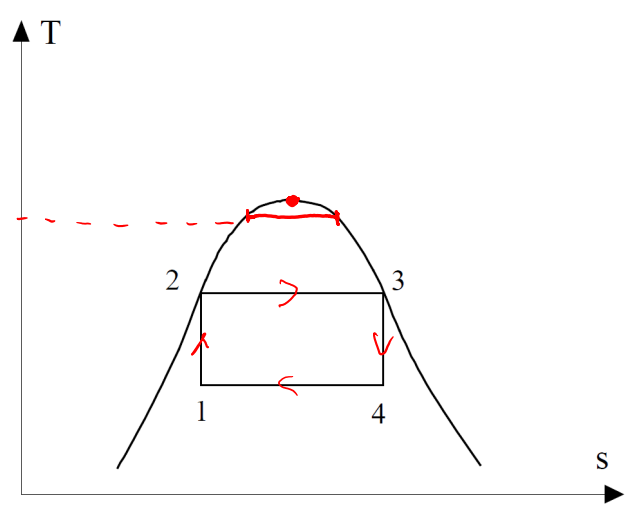
\includegraphics[height=4cm]{../L08/img1.PNG}
\end{center}
\textbf{Vantaggi}: 
\begin{itemize}
    \item Ricordiamo che se in zona bifase abbiamo temperatura costante (nelle isoterme) allora anche la pressione è costante. Ciò comporta che le isoterme siano anche isobare e dal punto di vista pratico le isobare sono facili da realizzare nella realtà.
    \item Un altro vantaggio di usare il ciclo di Carnot nella zona bifase è che c'è un notevole incremento di variazione di entalpia (dovuta all'entalpia di transizione), per cui se si guardasse l'area sottesa nel siagramma pressione-volume vedremmo che il lavoro specifico è alto.
\end{itemize}
\textbf{Svantaggi}:
\begin{itemize}
    \item E' molto dispendioso e difficile da realizzare la compressioen $1-2$.
    \item L'espansione $3-4$ è conveniente se il titolo $x_4 > 0,9$.
\end{itemize}
\subsubsection{Caratteristiche di un fluido di lavoro per il ciclo a vapore}
Per ridurre, a parità di potenza, la portata di fluido e quindi le dimensioni (e il costo) dell'impianto:
\begin{itemize}
    \item Elevata \textbf{massa volumica};
    \item Elevata \textbf{entalpia di transione di fase};
\end{itemize}
Al punto critico l'entalia di evaporazione è nulla:
\begin{itemize}
    \item Elevata \textbf{temperatura critica};
\end{itemize}
Evitare la presenza di una fase solida:
\begin{itemize}
    \item Temperature del \textbf{punto triplo} inferiore alla temperatura minima del ciclo;
\end{itemize}
Ridurre costi materiali e allungare ciclo di vita dell'impianto:
\begin{itemize}
    \item Fluido \textbf{non corrosivo};
\end{itemize}
Ridurre rischi ambientali:
\begin{itemize}
    \item Fluido \textbf{non tossico};
\end{itemize}
Aumentare sicurezza dell'impianto:
\begin{itemize}
    \item Fluido \textbf{chimicamente stabile};
\end{itemize}
Ridurre i costi:
\begin{itemize}
    \item Facilmente \textbf{reperibile e di basso costo};
\end{itemize}
Vapore in uscita dalla turbina con elevato titolo:
\begin{itemize}
    \item \textbf{Elevata pendenza} nel piano $T-s$ della curva limite superiore (più la curva è pendente e più il titolo allo stato $4$ sarà elevato);
\end{itemize}
Evitare infiltrazioni di gas incondensabili e conseguente necessità di apparecchiature atte al mantenimento dell'opportuno grado di vuoto (la temperatura al condensatore deve essere vicina a quella del serbatoio di calore inferiore per avere una limitazione delle irreversibilità):
\begin{itemize}
    \item \textbf{Pressione di condensazione} superiore alla pressione atmosferica;
\end{itemize}
\ \newline
\textbf{Nessun fluido} possiede tutte le proprietà citate. il fluido più adatto dipende dalle condizioni di contorno, in particolare delle temperatura delle sorgenti.\newline
\newline
\textbf{Cicli motore}: Tipicamente viene usata l'acqua che possiede le principali proprietà.\newline
\newline
\textbf{Cicli inversi (frigoriferi)}: Ci sono molti fluidi fra cui scogliere, per esempio:
\begin{itemize}
    \item Ammoniaca $NH_3$ (ma è tossico);
    \item Clorofluorocarburi (CFN o freon) (ma sono dannosi per l'ozono) (esempi: R11, R12);
    \item Clorofluoroidrocarburi (HCFC) e Fluoroidrocarburi (HFC) (sono meno dannosi per l'ozono) (esempi: R22, R123, \textbf{R134a})
\end{itemize}
\ \newline
Vediamo una tabella che mostra le caratteristiche di acqua e R134a, i due fluidi che useremo in questo corso:
\begin{center}
    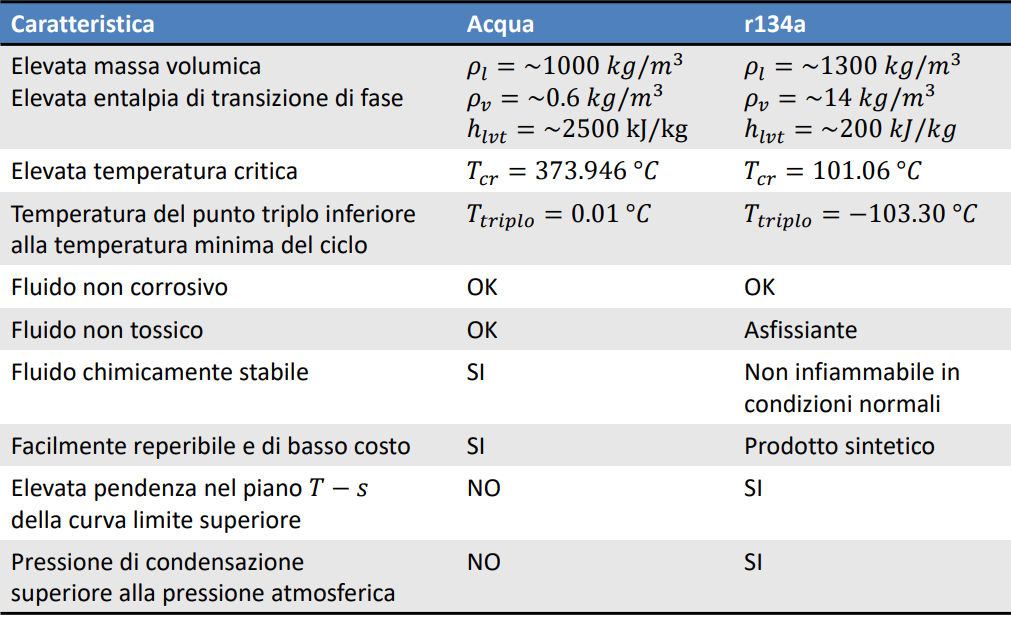
\includegraphics[height=6cm]{../L08/img2.PNG}
\end{center}
Vediamo ora i diagrammi $T-s$ (che possono anche essere usati al posto delle tabelle... le tabelle sono più precise):
\begin{center}
    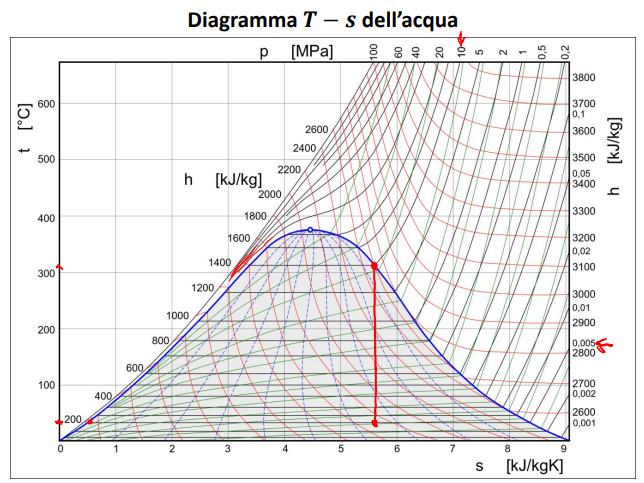
\includegraphics[height=5cm]{../L08/img3.PNG}
\end{center}
In azzurro: curva di saturazione, notiamo che la parte a destra di questa curva non è particolarmente ripida;\newline
Le curve nere sono le isobare, in cui si leggono le pressioni in mega pascal alcune in alto e alcune a destra;\newline
Tutte le righe orizzontali sono isoterme, e quelle verticali sono isoentropiche.\newline
Le curve rosse sono isoentalpiche (a parità di entalpia); \newline
Le curve verdi sono isovolumiche;\newline
Le curve azzurre tratteggiate sono quelle di isotitolo.
\begin{center}
    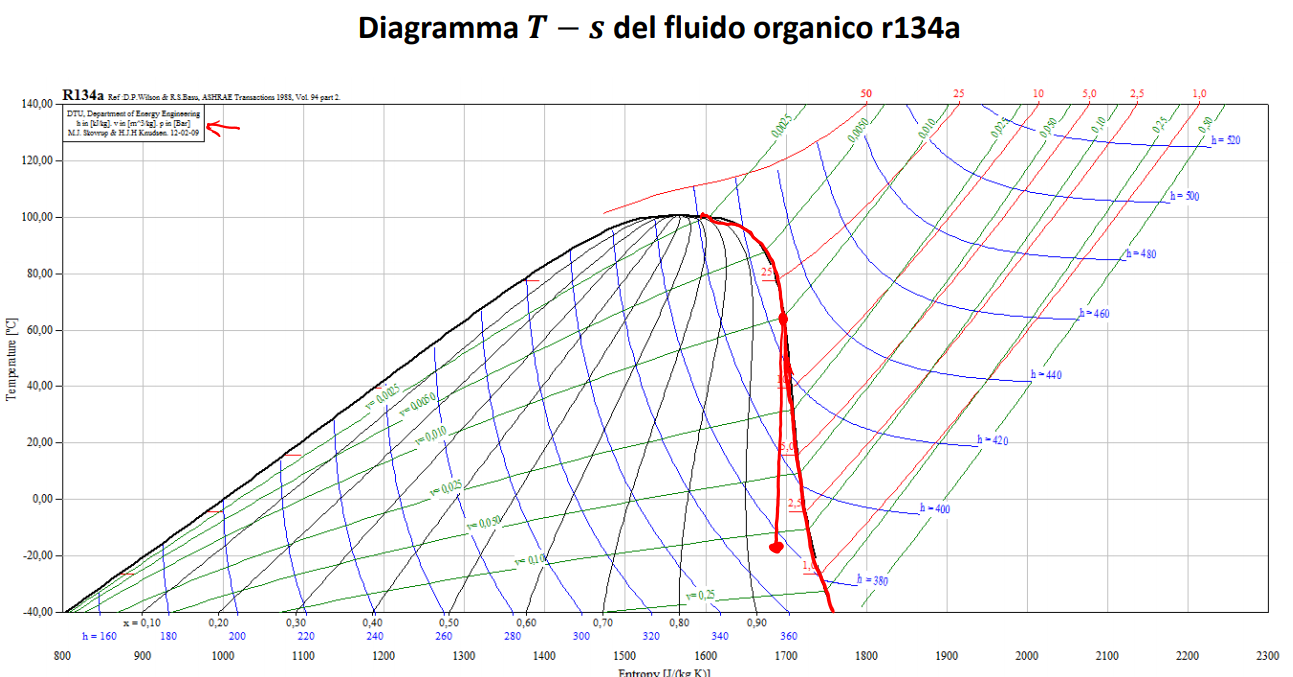
\includegraphics[height=5cm]{../L08/img4.PNG}
\end{center}
La curva nera marcata è la curva di saturazione: per l'r124a abbiamo una forte pendenza nella parte destra della curva di saturazione, questo vuol dire che si ha in uscita un alto titolo;\newline
Le curve verdi sono isovolumiche;\newline
Quelle in rosso sono isobare;\newline
Quelle azzurre sono le isoentalpie;\newline
quelle nere sono isotitolo;
\subsection{Ciclo Rankine}
\subsubsection{Ciclo Rankine semplice (a vapore saturo)}
Il ciclo Rankine semplice rappresenta un metodo per rendere realizzabile il ciclo di Carnot. La compressione $1-2$ nel ciclo di Carnot, all'interno del bifase, è un'operazione molto dispendiosa con molte irreversibilità interne. Per ovviare a questo porblema, viene fatta proseguire la condensazione fino allo stato $1$ della seguente immagine:
\begin{center}
    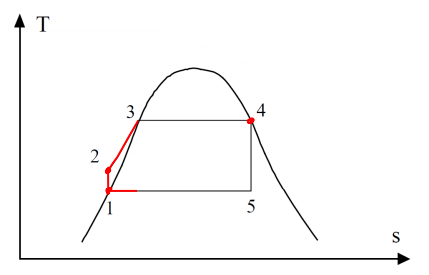
\includegraphics[height=4cm]{../L08/img5.PNG}
\end{center}
arrivati allo stato $1$ si ha un monofase liquido. Per far salire la pressione di questo liquido si usa ora una \textbf{pompa} fino a raggiugnere uno stato $2$.\newline
Nota: la rappresentazione della compressione $1-2$ non è fedele in quanto le isobare, nella zona dello stato liquido, sono molto vicine alla curva di saturazione (confrontare con il diagramma $T-s$ visto precedentemente). Per visualizzare meglio il ciclo spostiamo lo stato $2$ in modo che sia ben chiaro.
\begin{center}
    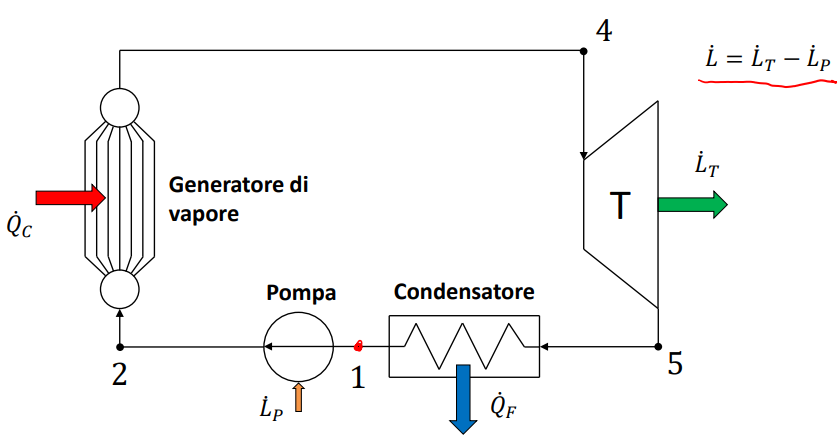
\includegraphics[height=5cm]{../L08/img6.PNG}
\end{center}
Arrivati allo stato $2$ si esegue una trasformazione isobara e si raggiunge lo stato $3$. le trasformazione $2-3$ e $3-4$ rappresentano lo scambiatore di calore, ma nel disegno dello schema di impianto, questo scambiatore di lavoro viene rappresentato come due cerchi collegati da una serie di connessioni. Questo componente è un generatore di vapore ed è posto in verticale perchè nel contenitore inferiore c'è acqua liquida, attraversando i vari tubi diventa vapore e giunge nel contenitore superiore. Per la gravità se ci fosse ancora acqua in stato liquido nel contenitore superiore, questa cadrebbe in modo da tornare a quello inferiore e ripetere il processo.\newline
\newline
Nell'espansione $4-5$ rimane il problema che il titolo in $5$ può essere minore di $0,9$ e quindi causare problemi (vedi svantaggi del ciclo di Carnot a vapore).\newline
\newline
Il lavoro totale uscente è il lavoro prodotto dalla turbina meno il lavoro che si spende nella pompa.
\subsubsection{Ciclo Rankine}
Il ciclo Rankine completo presenta una modifica ulteriore: per evitare di avere problemi di titolo minore di $0,9$ allo stato $5$ (all'uscita della turbina) ed aumentare il rendimento, si effettua il surriscaldamento del vapore $(4-5)$:
\begin{center}
    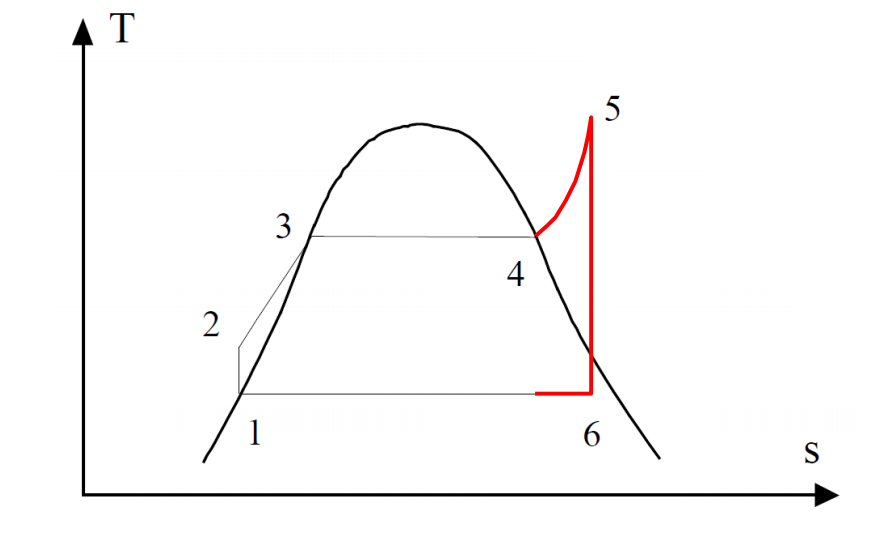
\includegraphics[height=4cm]{../L08/img7.PNG}
\end{center}
Notiamo che da $2$ a $5$ si è sulla stessa isobara: la pressione su $2,3,4,5$ è la stessa.\newline
\newline
L'espansione della turbina avviene quindi in $5-6$ e lo stato $6$ (cioè l'uscita della turbina) avrà un titolo maggiore rispetto al caso di ciclo Rankine semplice.\newline
\newline
Questo riscaldamento aggiuntivo aumenta la potenza erogata dalla turbina (si ha un salto entalpico maggiore fra $5-6$), ma dall'altro lato si avrà una spesa maggiore, ma comunque si avrà un rendimento più alto
\[
    \eta = 1- \frac{\dot{Q}_F}{\dot{Q}_C} = 1- \frac{h_6-h_1}{h_5-h_2}
\]
\ \newline
Dal punto di vista impiantistico la differenza è che il flusso in uscita dal generatore di vapore viene deviato verso il generatore di vapore in modo da rimetterlo a contatto con una fonte di calore.
\begin{center}
    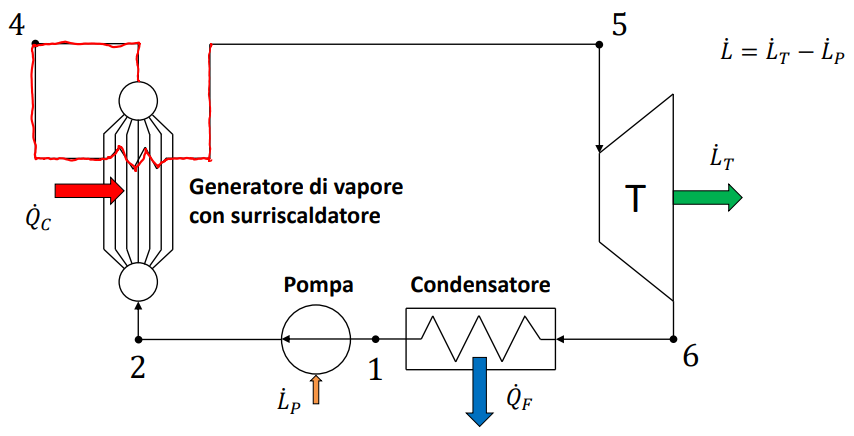
\includegraphics[height=5cm]{../L08/img8.PNG}
\end{center}
\ \newline
\textbf{Soluzioni per migliorare il rendimento del ciclo Rankine}\newline
\begin{itemize}
    \item \textbf{Riduzione della pressione di condensazione}:\newline
    Cioè si cerca di portare la temperatura nel condensatore a quella dell'ambiente (cioè la sorgente di calore inferiore), ovvero stiamo cercando di abbassare la trasformazione $6-1$.
    \begin{center}
        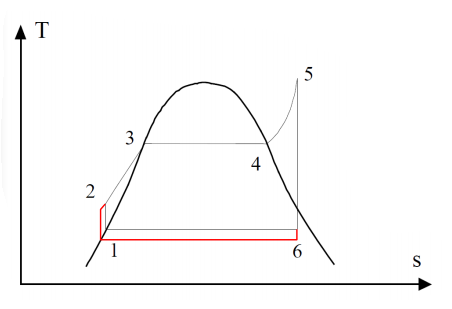
\includegraphics[height=3cm]{../L08/img9.PNG}
    \end{center}
    Nel condensatore se si abbassa la temperatura di saturazione si abbassa anche la pressione.\newline
    \newline
    Il limite principale di questo miglioramente sono i limiti tecnologici: limiti tecnologici per le infiltrazioni quando $P < P_{atm}$ (tipico quando si utilizza acqua)..\newline
    \newline
    Siccome si ha una differenza di temperatura maggiore nella trasformazione della turbina, allora si ha un aumento del lavoro prodotto, contemporaneamente si avrà anche un innalzamento del consumo della pompa, ma la turbina produce di più di quanto la pompa consumi.\newline
    \newline
    Avremo tendenzialmente un rendimento del ciclo maggiore, ma anche un rendimento della macchina termica migliore (si diminuiscono le irreversibilità esterne).
    \item \textbf{Aumento della temperatura finale di surriscaldamento}:\newline
    \begin{center}
        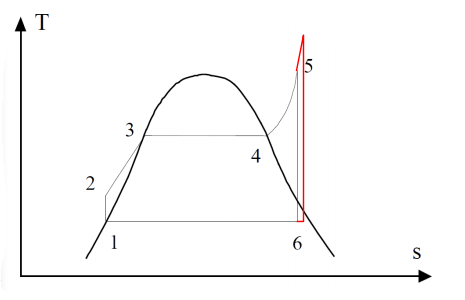
\includegraphics[height=3cm]{../L08/img10.PNG}
    \end{center}
    Si aumenta la temperatura massima del ciclo, in modo che aumenti il salto entalpico della turbina e quindi aumenti il lavoro prodotto. Il lavoro prodotto dalla turbina è maggiore della quantità di calore necessaria da fornire e quindi si ha un miglioramento del rendimento.\newline
    \newline
    Inoltre si ha pure un aumento del titolo d'uscita dalla turbina. \newline
    \newline
    I limiti dell'aumento della temperatura sono di tipo tecnologico ($T_{max} = 650^o C$).
    \item \textbf{ Aumento della pressione di vaporizzazione}:\newline
    Questo consente di ridurre la potenza termita scambiata a parità di produzione di energia meccanica della turbina.
    \item Surriscaldamenti ripetuti.\newline
    Nel ciclo Rankine ne abbiamo solo uno di surriscaldamento, ma se ne possono fare di più.
    \item \textbf{Rigenerazione}:\newline
\end{itemize}